\documentclass[aspectratio=169,10pt]{beamer}
\usetheme{Madrid}
\usepackage{graphicx}
\usepackage{amssymb}

% Tắt shadow
\setbeamertemplate{blocks}[rounded][shadow=false]
\setbeamertemplate{navigation symbols}{}

% Color configuration
\definecolor{primaryblue}{RGB}{20, 55, 110}
\setbeamercolor{palette primary}{bg=primaryblue,fg=white}
\setbeamercolor{structure}{fg=primaryblue}

\begin{document}

\begin{frame}{Graph in $\mathbb{R}^3$ and Level Curves}
    \begin{columns}[T]
        % Cột trái: 2 Khung định nghĩa và phương pháp vẽ
        \begin{column}{0.56\textwidth}
            \begin{block}{Definition (Graph in $\mathbb{R}^3$)}
                \small
                The \textbf{graph} of function $z = f(x, y)$ with domain $D$ is:
                \[
                    \{(x, y, z) \in \mathbb{R}^3 \mid (x, y) \in D \text{ and } z = f(x, y)\}.
                \]
                It is a \textbf{surface} defined by the function.
            \end{block}

            \vspace{0.1cm}

            \begin{block}{Question: How can we plot a surface?}
                \small
                \begin{itemize}
                    \item For $s = g(t)$, we connect sample points with a smooth curve.
                    \item For $z = f(x, y)$, this fails. Instead, for each $z = z_0$, draw the \textbf{level curve} $z_0 = f(x, y)$.
                    \item This is the \textbf{intersection} of the surface and horizontal plane $z = z_0$:
                    \[
                        L_{z_0} := \{(x, y) \mid f(x,y) = z_0\}.
                    \]
                \end{itemize}
            \end{block}
        \end{column}

        % Cột phải: Animation trực quan hoá mặt phẳng cắt
        \begin{column}{0.42\textwidth}
            \centering
            \vspace{0.15cm}
            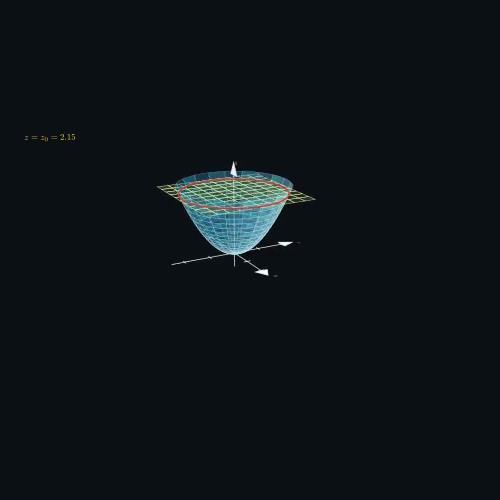
\includegraphics[width=0.92\linewidth, keepaspectratio]{SurfaceLevelCurvesScene.png}
            
            \vspace{0.1cm}
            {\tiny \textcolor{gray}{\textit{Slicing $z = f(x, y)$ with horizontal plane $z = z_0$ to obtain level curves}}}
        \end{column}
    \end{columns}
\end{frame}

\end{document}
